\section{Userlib Schnittstelle}



\begin{frame}{Userlib}
    \begin{Large}
        Userlib als Grundlage für Schnittstelle
    \end{Large}
    \vspace{15pt}

    \begin{itemize}
        \item Kapselung des Kernels
        \item Apps nur gegen Userlib
        \item Verbindung zu Kernel via Syscalls
    \end{itemize}
    
\end{frame}


\begin{frame}{Userlib}
    \begin{Large}
        $\Rightarrow$ Beide Kernel implementieren Userlib \newline \newline
        $\Rightarrow$ Apps laufen unabhänging
    \end{Large}
    \vspace{15pt}
\end{frame}


\begin{frame}{Userlib Erweiterung}
    \begin{Large}
        Erweiterung der lib: {\tiny \cite{usrlib-repo}}
    \end{Large}
    \vspace{15pt}

    \begin{itemize}
        \item mehr Syscalls
        \item wrapper um die Syscalls
        \item Musik
        \item Bilder
        \item System Management
    \end{itemize}
\end{frame}


\begin{frame}{Userlib Aufbau}
    \begin{Large}
        Aufbau: \tiny \cite{usrlib-repo}
    \end{Large}
    \vspace{5pt}
    

    \begin{minipage}[t]{0.48\textwidth}
        \centering
        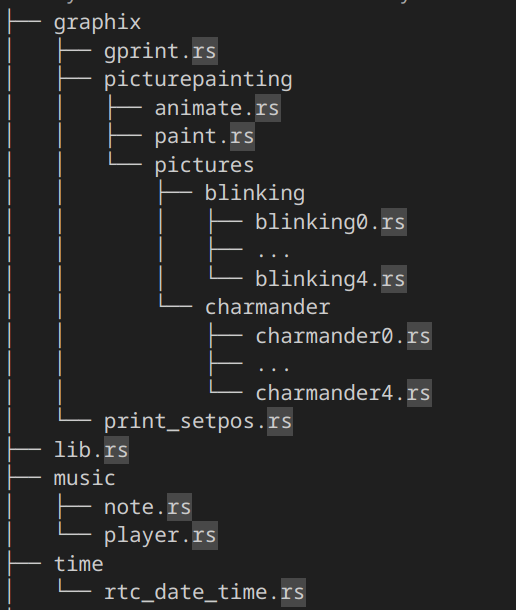
\includegraphics[height=0.7\textheight]{fig/Code Screens/Tree 1.png} 
    \end{minipage}
    \hfill
    \begin{minipage}[t]{0.48\textwidth}
        \centering
        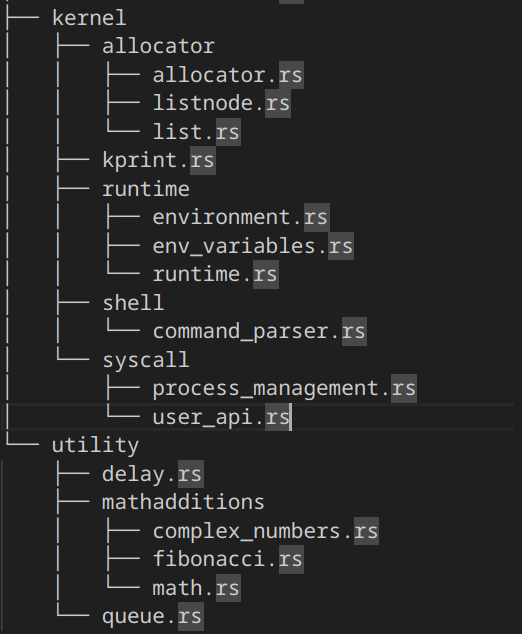
\includegraphics[height=0.7\textheight]{fig/Code Screens/Tree 2.png} 
    \end{minipage}
\end{frame}



\begin{frame}{Userlib Aufbau}
    \begin{minipage}[t]{0.3\textwidth}
        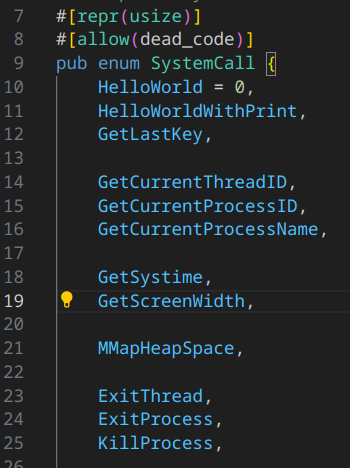
\includegraphics[height=0.8\textheight]{fig/Code Screens/Enum1.png} 
    \end{minipage}
    \hfill
    \begin{minipage}[t]{0.65\textwidth}
        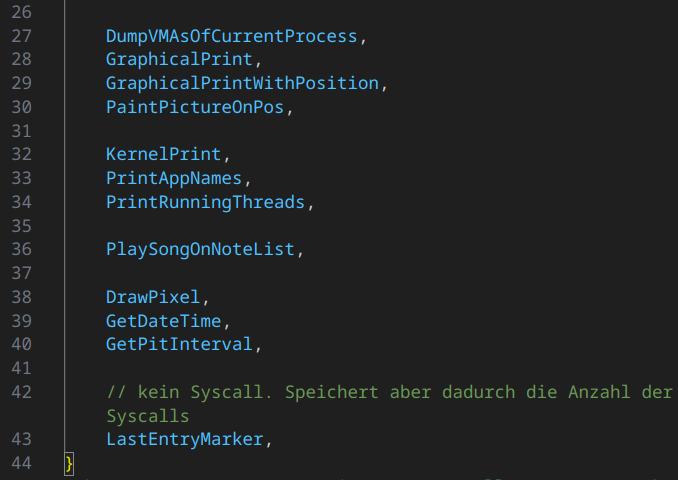
\includegraphics[height=0.8\textheight]{fig/Code Screens/Enum2.png} 
    \end{minipage}
\end{frame}